\documentclass[11pt,leqno]{article}

%\usepackage{comment}
\usepackage{amsfonts}
%\usepackage{latexsym}
\usepackage{amssymb}
\usepackage{amsmath}
\usepackage{graphicx}
\usepackage{float}
\usepackage{epstopdf}
%\usepackage{parskip}

%\setlength{\textwidth}{6.2in}
%\setlength{\oddsidemargin}{0.2in}
%\setlength{\evensidemargin}{0in}
%\setlength{\textheight}{8.9in}
%\setlength{\voffset}{-1.0in}
%\setlength{\parindent}{20pt}
%\setlength{\parindent}{1cm}
\setlength{\textwidth}{6.2in}
\setlength{\oddsidemargin}{0in}
\setlength{\evensidemargin}{0in}
\setlength{\textheight}{9in}
\setlength{\voffset}{-.9in}
\setlength{\headsep}{26pt}
%\setlength{\mathindent}{1cm}


\newcommand{\beq}{\begin{equation}}
\newcommand{\eeq}{\end{equation}}

\newcommand{\ba}{\begin{array}}
\newcommand{\ea}{\end{array}}

\newcommand{\bea}{\begin{eqnarray}}
\newcommand{\eea}{\end{eqnarray}}

\newcommand{\p}{\partial}
\newcommand{\pp}[2]{\frac{\partial #1}{\partial #2}}
\newcommand{\ppn}[3]{{\partial^{#1} #2 \over \partial #3^{#1}}}
\newcommand{\Pain}{Painlev\'{e} }

\newcommand{\mbf}[1]{\mbox{\boldmath {$#1$}}}
\newcommand{\tx}{\mbox}

\newcommand{\ol}{\overline}
\newcommand{\ft}{\widehat}
\newcommand{\mb}{\mathbb}

%\setlength{\parskip}{2mm}
\renewcommand{\theenumi}{\alph{enumi}}
\renewcommand{\labelenumi}{(\theenumi)}

\begin{document}

%\begin{center}
\title{\bf Adaptive Mesh Refinement for 1-D Hyperbolic PDEs}
\author{ 
Saumya Sinha\footnote{Department of Applied Mathematics, University of Washington, Seattle, Washington
U.S.A.
Email:\texttt{saumya@uw.edu}},
Kenneth J. Roche\footnote{
High Performance Computing Group, 
Pacific Northwest National Laboratory,
1 Battelle Road,
Richland, Washington 
U.S.A. 
Email:\texttt{kenneth.roche@pnnl.gov}} 
}
\maketitle
%\end{center}


{\small {\bf \abstractname}{: We describe an adaptive mesh refinement algorithm that extends high resolution wave-progpagation techniques to hyperbolic systems in non-conservative form. The method for keeping numerical conservation at grid cell interfaces is described. The algorithm was tested for simple 1D problems. Results are compared to static mesh solutions for the same problems computed with Clawpack\cite{claw}.}}


\tableofcontents
\listoffigures
\listoftables
\newpage

\section{Overview of Paper}
An adaptive mesh refinement strategy that uses rectangular patches over Cartesian grids to refine both space and time coordinates is useful for modeling and tracking regions where the solutions are not smooth such as exhibited around shocks. We present an AMR algorithm in the next section, and provide details in subsequent sections for the various steps. 

\section{Pseudo-code for AMR}
\noindent Steps for the AMR algorithm:
\begin{enumerate}
\item{initialize coarse grid}
\item{evolve time on coarse grid}
\item{{\it recurse}: estimate error, create fine grid}
\begin{itemize}
\item{cell flagging}
\item{clustering}
\item{fine grid generation}
\end{itemize}
\item{solve Riemann on refined grid levels}
\item{correction step to ensure conservation}
\item{go to step {\it b} }
\end{enumerate}

\subsection{wave propagation algorithm to evolve time}
After initializing the discrete coarse grid, a standard high resolution wave propagation including limiter corrections to evolve our Riemann problem is employed. The method reads,  i.e. for the {\it color} eqn (see \ref{color}):
\begin{equation} \label{hires}
 q_{i}^{n+1} = q_{i}^{n} - \frac{k}{h}(u_{i}^{+}(q_{i}^{n}-q_{i-1}^{n})+u_{i}^{-}(q_{i+1}^{n}-q_{i}^{n})) - \frac{k}{h}(\tilde{F_{i+1}} - \tilde{F_{i}})
 \end{equation}
 \noindent where 
 \begin{equation}
\tilde{F_{i}} = \frac{1}{2}\vert u_i \vert (1- \frac{k}{h}\vert u_i \vert) \tilde{W_i}
 \end{equation}
 \noindent and the limiter is applied to wave $W_i = q_i - q_{i-1}$ i.e. traveling at speed $u(x)$, such that
\begin{equation}
 \tilde{W_i} =
  \left\{ \begin{array}{c}
limiter(W_i , W_{i-1}) , \, \, \, \, u_i > 0\\
limiter(W_i , W_{i+1}) , \, \, \, \, u_i < 0\end{array}\right 
\end{equation}
Clearly, when $\tilde{W_i} = W_i$ the method is reduced to upwind + second order correction, i.e. Lax-Wendroff method. 
On notation: $h,k$ are mesh spaces for the coarse coordinate and time grids respectively, and $u^+ (x) = max(u(x),0)$ and $u^- (x)=min(u(x),0)$ at $x$.

\subsection{determining refinement - error estimation}\label{whentorefine}
The idea behind the refinement step comes from first determining where a refinement may be useful.  
If the solution $q(x,t)$ is smooth enough, we assume that method $D$ (application of eqn(\ref{hires})) has accuracy $O(s)$ in both 
space and time. The local truncation error is $q(x,t+k) -D q(x,t) = \tau(x,t) + k O(k^{s+1}+h^{s+1}))$ where $\tau$ is the leading error.
Taking two time steps suggests $q(x,t+2k) -D^2 q(x,t) = 2\tau(x,t) + k O(k^{s+1}+h^{s+1}))$.
Now, coarsen the grid to have space and time widths $2h$, $2k$ and let the differencing scheme be called $D_{2h}$ in this case. The local truncation error in this case reads $q(x,t+2k) -D_{2h} q(x,t) = 2^{s+1}\tau(x,t) + O(h^{s+2})$. Thus, an error growth estimate at time $t$ can be formed by taking the difference in the error taking two steps with the regular integration scheme, and a single large step using every other grid point:
\begin{equation}
\frac{D^2 q(x,t) - D_{2h} q(x,t)}{2^{s+1}-2} = \tau(x,t) + O(h^{s+2}) \, .
\end{equation}
The difference between the solutions obtained on the two grids at each point is proportional to the local truncation error at that point. At coarse cells where the difference between the two sets of values exceed some tolerance, all four cells contained in the real grid are flagged as requiring refinement. See \cite{berg-coll} for more details. {\it Clustering} is simply to fill gaps in neighboring cells flagged for refinement. Should there be a cell not flagged for refinement between cells that require refinement, the cell in between will be refined as well because in the next step it is likely refinement will be required. A buffer zone around the flagged cells is added to track features of interest in the refined region. This buffer zone must be affiliated with the number of time steps evaluated at a particular level. If a patch at level $L$ is refined by even integer $R_L$, then the time-step is equally refined implying that $R_L$ steps must be taken on the refined grid at level $L+1$ for each step on grid at level $L$. 

\subsection{assigning values to new fine grid points}
Once regions where a fine grid are determined, values must be assigned to the fine grid points. Space-time interpolation is needed to supply values for the fine grid because more time steps are taken on the fine grid  than the coarse grid and there are no coarse grid values available at intermediate times. 
This is achieved through a linear interpolation step with known coarse grid values and these values are available since we advance the coarse grid first as stated in the algorithm.

\subsection{flux updates on refined and coarse meshes}
After finishing the recursive step creating the fine grid structure, how to evolve the newly refined grid needs to be considered. To evolve, conservation of fluxes at grid interfaces is required. We refer to Fig \ref{fig21} for this discussion. There are essentially three cases to consider: coarse cell to coarse cell, fine cell to fine cell, and overlapping coarse cell and fine cell regions. Let $F_i$ be the flux at the left edge of coarse cell $i$. This is different notation than what we typically wrote in class, $F_{i-\frac{1}{2}}$. 
\begin{figure}[h]
    \centering
    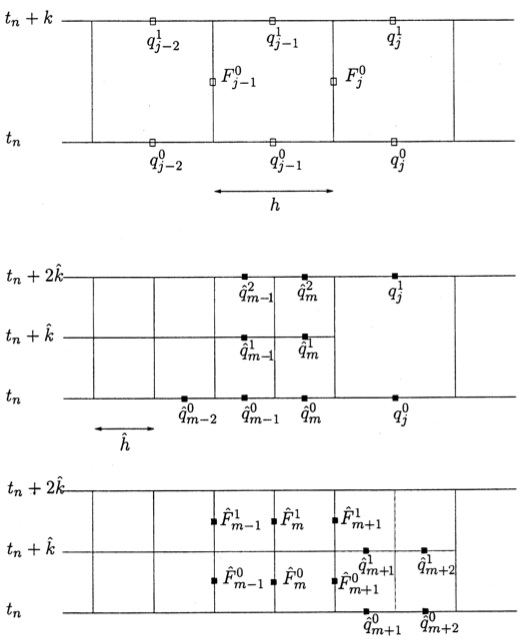
\includegraphics[width=.6\textwidth]{berg-lev-fig21}
   \caption{Essential figure for flux adapting Cartesian grids. The top grid is the normal coarse grid we are used to using with fluxes indicated. The middle diagram shows the case where a fine grid overlays a coarse grid and the interface region of fine and coarse grids. Recall that $2\hat{h}=h$ and $2\hat{k}=k$. The bottom diagram depicts the ghost cell region imposed on the coarse cell interface as well as the fine grid fluxes needed to bridge the interface.}
    \label{fig21}
\end{figure}

Updating between coarse grid cells is, to lowest order, simply:
\begin{equation}
q_{i}^{1} = q_{i}^{0} - \frac{k}{h} (F_{i+1}^{0} - F_{i}^{0}) 
\end{equation}
\noindent where $h,k$ are the space and time lattice spacing respectively.

In regions that contain $m$ adjacent single level refined cells let the lattice spacing be denoted by $\hat{h},\hat{k}$.
We have, in the stated order, $\forall i=1,m$
\begin{equation}
\begin{array}{c}
\hat{q}_{i}^{1} = \hat{q}_{i}^{0} - \frac{\hat{k}}{\hat{h}} (\hat{F}_{i+1}^{0} - \hat{F}_{i}^{0}) \\
\hat{q}_{i}^{2} = \hat{q}_{i}^{1} - \frac{\hat{k}}{\hat{h}} (\hat{F}_{i+1}^{1} - \hat{F}_{i}^{1}) 
\end{array}
\end{equation}
\noindent in the refined cells where we assume each refinement is $2X$.

In regions where the coarse and fine grids overlap, care must be taken. Two ghost cells are introduced, $\hat{q}_{m+1},\hat{q}_{m+2}$. The values in these 
cells are decided by evaluating a polynomial (determined by interpolating the coarse values $q_{i}^{0}, q_{i}^{1}$)  at these fine grid locations. At the final time (completed time step)  $q_{i}^{1}$ is replaced by the average of the 
fine grid values in the overlapped region:
\begin{equation}
q_{j-1}^{1} = \frac{1}{2} (\hat{q}_{m+1}^{2}+\hat{q}_{m+2}^{2})
\end{equation}
\noindent and the corresponding left edge flux is similarly modified so that $q_{i}^{1}$ is finally modified as:
\begin{equation}\label{fluxcorrect}
q_{i}^{1} \rightarrow q_{i}^{1} + \frac{k}{h} ( \frac{1}{2}(\hat{F}_{m+1}^{0} + \hat{F}_{m+1}^{1}) - F_{i}^{0}) \, .
\end{equation}
 
 
 
\subsection{updating grid interfaces with wave propagation -correction step}
With flux-differencing to ensure conservation, a new coarse grid value is updated by an average of fine-grid values in any cell covered by a fine grid. The key to conservation is that flux into coarse cells is accounted for by flux out of adjacent fine cells, and vice versa, as described in the previous section. Wave propagation algorithms are written in a manner that they can be extended to hyperbolic problems not in conservation form retaining wave features but with no flux function. 
For wave-propagation algorithms, a similar correction is needed for the waves to yield conservation.  The wave-propagation form can be used to update the values at the interface between fine and coarse grid cells on each grid independently using �ghost-cell� values as needed near grid interfaces.

Recall from class that $A^+ \Delta q_{i-\frac{1}{2}}$ measures the net effect of all right going waves present from $x_{i-\frac{1}{2}}$, and $A^- \Delta q_{i-\frac{1}{2}}$ measures the net effect of all left going waves from the same interface. We call these {\it fluctuations}.
Whether conservative or non-conservative systems are treated, second-order corrections are still written as flux-differences. 
However, the first-order upwind terms written in terms of the fluctuations must be handled differently. 
To maintain conservation we must {\it first} solve the Riemann problem between the ghost cell value $\hat{q}_{m+1}^{0}$ on the fine grid and the coarse grid value $q_{j}^{0}$, and add to the coarse cell value $q_{j}^{1}$ the resulting total fluctuation (dropped indices) $A^{-}\Delta q + A^{+}\Delta q$ weighted by $\hat{k}/h = 1/2$ since the time step is $\hat{k}$ while the cell size is $h$. 
{\it Second} we must also solve a Riemann problem on the fine grid between $\hat{q}_{m+1}^{1}$ and $q_{j}^{0}$
and add these fluctuations into $q_{j}^{1}$. 

The correction step extends to an arbitrary hyperbolic system (i.e. see \ref{linsys} for linear hyperbolic system of PDEs) where we use a Riemann solver to obtain $A^{-}\Delta q$ and  $A^{+}\Delta q$ from the two states $\hat{q}_{m+1}^{0}$ and $q_{j}^{0}$.  This step is made in each of the $R$ time steps on the refined grid within the single coarse-grid step, where $R$ is the refinement ratio. \\

\noindent In summary, the correction algorithm reads:
\begin{description}
  \item[for $N = 0 , R-1$] \hfill \\
  solve the Riemann problem with data $\hat{q}_{m+1}^{N}$ and $q_{j}^{0}$ to compute $A^{-}\Delta q$ and  $A^{+}\Delta q$\\ \hfill
  update $q_{j}^{1} \rightarrow q_{j}^{1} + \frac{\hat{k}}{h}$ ($A^{-}\Delta q + A^{+}\Delta q$)
\end{description}


\subsection{Note on boundary conditions}

\section{Examples of 1D AMR}
\subsection{variable coefficient}\label{color}
Here we state a 1D scalar problem based on a variable coefficient velocity term.The {\it color} equation is the problem formed by solving the following Riemann problem at the interface $x_{i-\frac{1}{2}}$ between cells $i-1$ and $i$:

\begin{equation}
 q(x,t)_{t} + u(x) q(x,t)_{x}=0
 \end{equation}

\begin{equation}
q(x,0):= \phi(x)=
\left\{ \begin{array}{c}
q_{i-1} , \, \, \, \, x<x_{i-\frac{1}{2}}\\
q_{i} , \, \, \, \, x>x_{i-\frac{1}{2}}\end{array}\right
 \quad 
,
\quad u(x)=
 \left\{ \begin{array}{c}
u_{i-1} , \, \, \, \, x<x_{i-\frac{1}{2}}\\
u_{i} , \, \, \, \, x>x_{i-\frac{1}{2}}\end{array}\right 
\end{equation}
\noindent and the sign of $u(x)$ arbitrary for now.

\subsection{linear system (acoustics)} \label{linsys}
We study here the 1D systems of the form
\begin{equation}
q(x,t)_{t} + A q(x,t)_{x}=0
\end{equation}
\noindent and $A$ satisfies hyperbolicity conditions.

\section{Results}
\subsection{Software implementation}
Clawpack was used to generate numerical Riemann solutions to our test problems for the fixed mesh case.
We utilized (Python, Matlab, C) for our AMR implementations.
Please find our software here: (need software + examples ...) and use the \texttt{Readme.txt} file there 
to build and test the software. The test cases presented in this report are reproduced there.
\subsection{Results of the Numerical experiments for the 1D cases}

\section{Summary}
In this paper we described the adaptive mesh refinement algorithm presented in \cite{Berger1998}, and tested the 
algorithm for several simplistic 1D cases. Our results were compared against those from Clawpack. Our AMR 
implementations are available to anyone who wants them.

\begin{thebibliography}{9}
\bibitem{claw}
http://www.clawpack.org\\

\bibitem{levFVMHP}  
  R.~Leveque
Finite Volume Methods for Hyperbolic Problems
 Cambridge University Press (2002)  \\

\bibitem{berg-coll}
M.~Berger and P.~Collela, Local Adaptive Mesh Refinement for Shock Hydrodynamics
Journal of Computational Physics 82, 64-84 (1989)\\

\bibitem{Berger1998}
M.~Berger and R.~Leveque, Adaptive Mesh Refinement Using Wave-Propagation Algorithms for Hyperbolic Systems
SIAM Journal of Numerical Analysis, 35(6):2298--2316, (1998)\\

\bibitem{Berger1982}
M.~Berger, Adaptive Mesh Refinement for Hyperbolic Partial Differential Equations,
 {\em PhD Thesis}, Department of Computer Science, Stanford University, Stanford, CA 94305 (1982)\\

\end{thebibliography}

\end{document}